\subsubsection{Evaluation of different levels of refinement for different number of cores}
This experiment is first run on CAPER cluster, with a maximum of 128 cores, from level 1 to level 4 on 2, 4, 8, 16, 32, 64 and 128 cores. The execution time is recorded simply with the system tool ``time''.

\noindent
\textbf{Configuration}
\begin{table}[H]
\begin{center}
\begin{tabular}{|l|l|}
	\hline
	\textbf{Parameter} & \textbf{Value}\\ \hline
    Platform & CAPER and DELL cluster\\ 		\hline
    Number of cores & 2 to 128 quadratic growth\\
	\hline
    Level of refinement  & level 1 to level 4\\
    \hline
    Time step & 10\\
    \hline
    Time unit & Second\\
    \hline
\end{tabular}
\end{center}
\caption{Configuration for experiment of execution time of different levels of refinement under variety number of cores
}
\label{table:table_time_refinement}
\end{table}


\noindent
%\textbf{Result}
\begin{figure}[H]
	\centering
    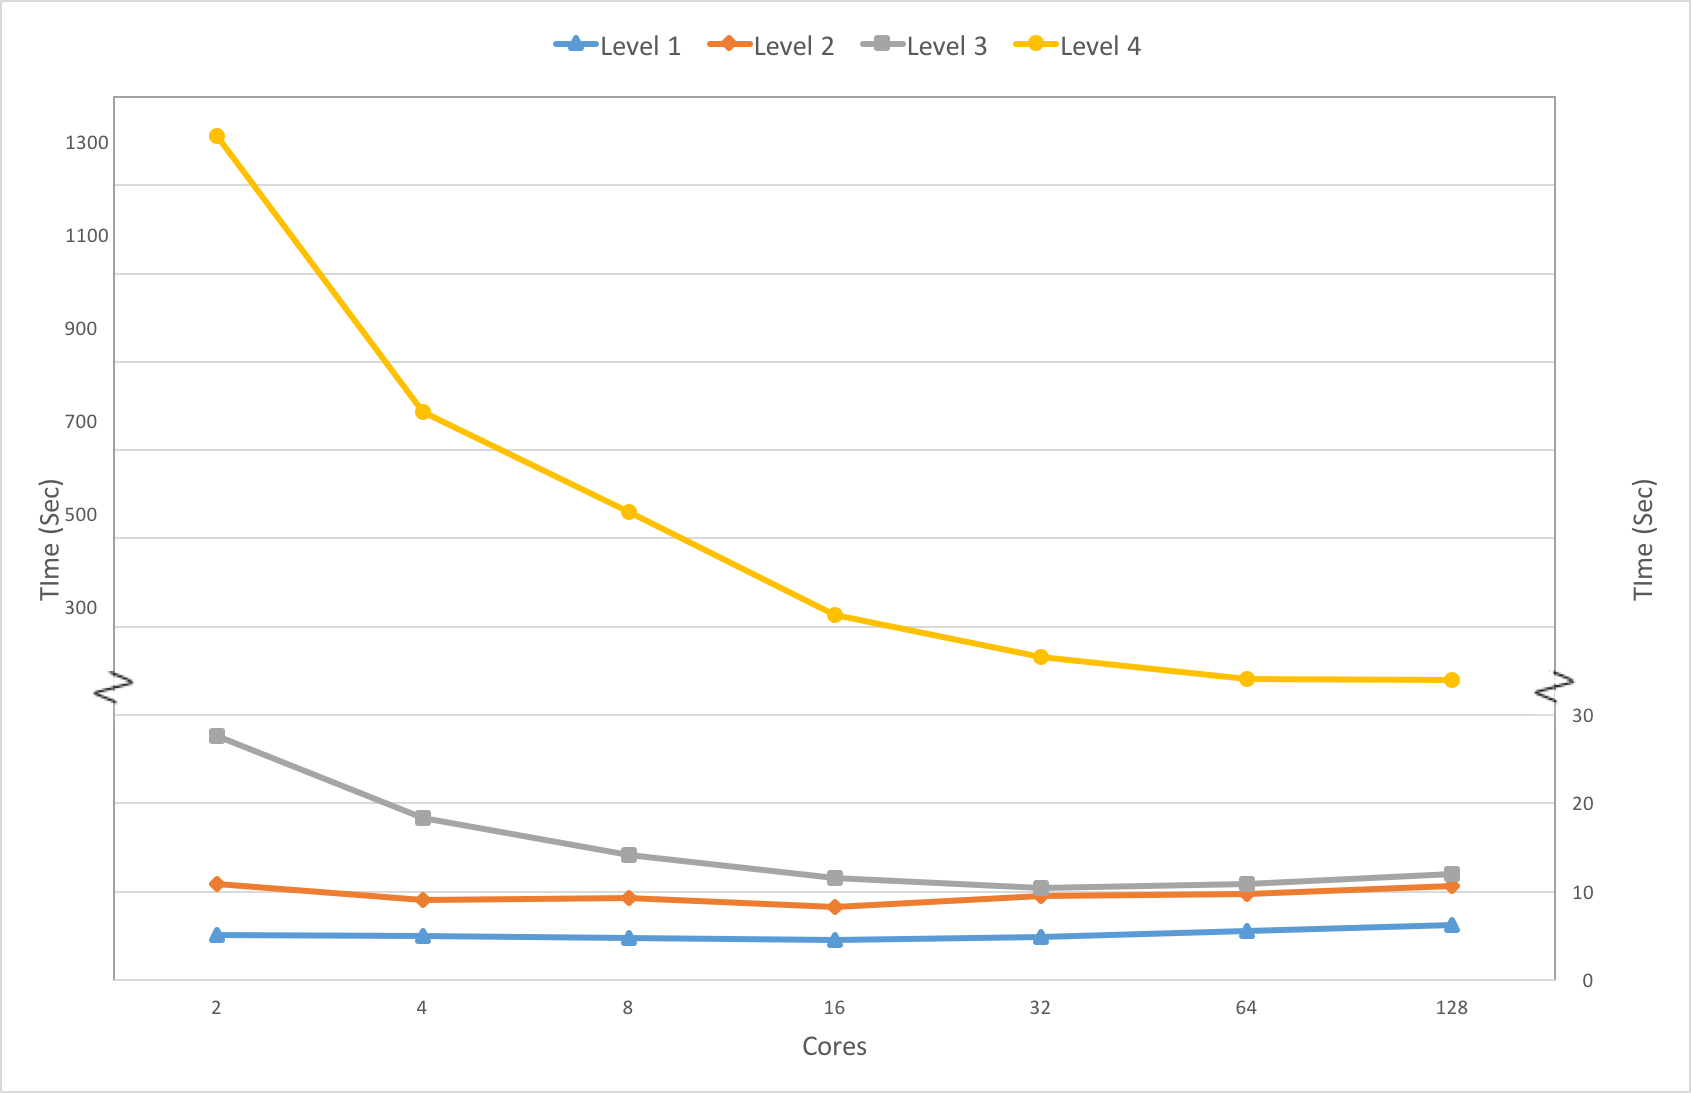
\includegraphics[width=8cm]{figs/CAPER_lev1-4_run_time_edited.jpg}
        \caption{Execution time of running different levels LMC on CAPER cluster through 2 to 128 cores. }
        \label{fig:executiontimeoncaper}
\end{figure}

\begin{figure}[H]
	\centering
    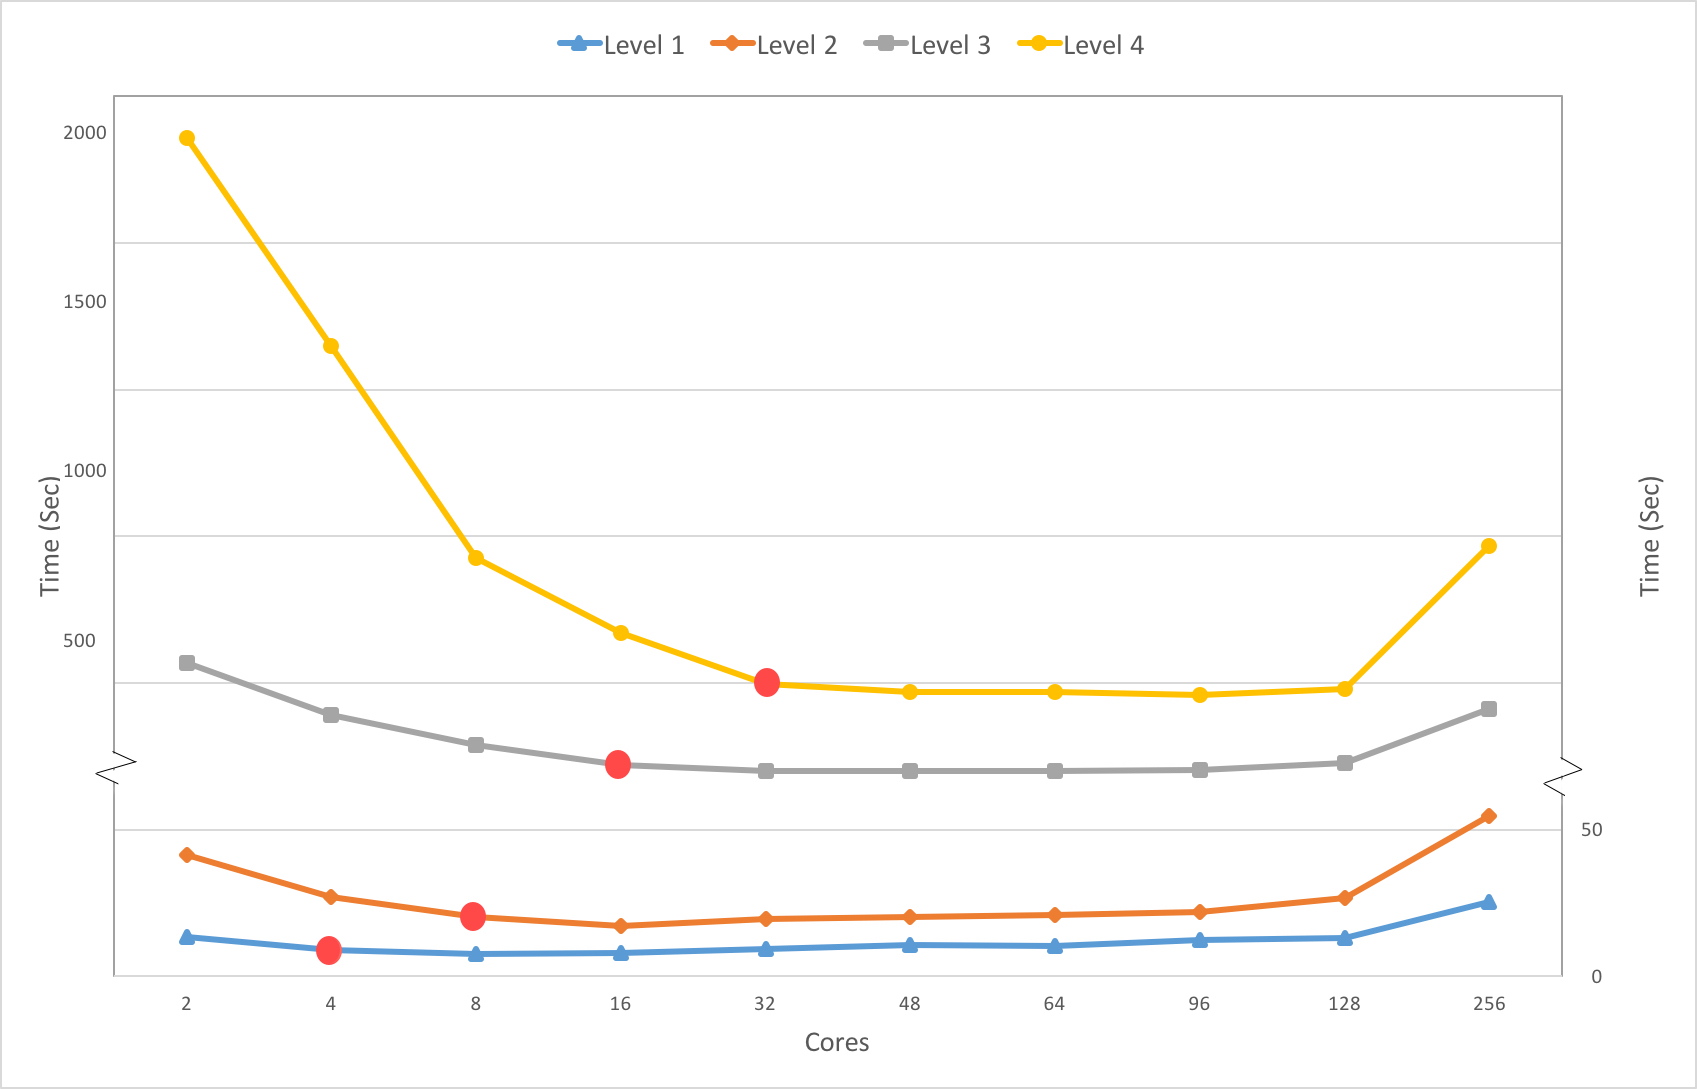
\includegraphics[width=8cm]{figs/Dell_lev1-4_run_time_edited.jpg}
        \caption{Execution time of running different levels LMC on DELL cluster through 2 to 256 cores. }
        \label{fig:executiontimeondell}
\end{figure}

%\noindent
%\textbf{Discussion}

The results of the first experiment using CAPER cluster are shown in Figure \ref{fig:executiontimeoncaper}. As can be clearly seen from the level 4 line, which is yellow line with solid dot maker, the more computing resource we use, the faster the execution is. Comparing these four lines, we can also notice that the slope is decreasing from level 4 to level 1, and then the lines go to a relative flat zoom. From this notice, we can see that heavier workload need more computational resources, but provisioning more resources do not bring any performance increase. In Figure \ref{fig:executiontimeoncaper} it can be seen from level 1 to level 3 lines that their tails are tilting a little bit, but level 4 line doesn’t have this trend. In order to show its trend more clearly, we ran this experiment on DELL cluster (256 cores cluster). The result is shown in Figure \ref{fig:executiontimeondell}. All levels' curve is like a ``U'', that tilt in the head and tile. From level 1 to level 4, the head turning point, which marked by red dot, are respectively 4, 8, 16 and 32 cores. Then they tend to get into a flat zoom, while under the 256 core, the execution time are all increase. From these two experiments we can conclude that, to achieve optimal running time, we need to configure appropriate number of processors to execute certain level of quality for the LMC program and using more processors does guarantee better performance.



\subsubsection{Evaluation of energy consumption of different levels of refinement under variety number of cores}
In this experiment, we are aim at exploring the energy consumption of running LMC with different level of refinement under multiple number of cores. 

%\noindent
%\textbf{Methodology}

Energy is the product of power and time, therefore, in this experiment, we need to measure the execution time and power respectively. To measure time, we still use Linux command TIME in the script file. And for the CPU power, we are using RAPL power meter to measure it. RAPL power meter is a sub-function of Intel Power Gadget program, which has been mentioned in previous background section. We are sampling power data every 0.5 second.

\noindent
\textbf{Configuration}
\begin{table}[H]
\begin{center}
\begin{tabular}{|l|l|}
	\hline
	\textbf{Parameter} & \textbf{Value}\\ \hline
    Platform & CAPER cluster\\ 		\hline
    Number of cores & 2 – 128 quadratic growth\\
	\hline
    Level of refinement  & level 1 to level 4\\
    \hline
    Time step & 10\\
    \hline
    Time unit & Second\\
    \hline
    Power measurement object & 8 nodes processors\\
    \hline
    RAPL sample rate & 2 Hz\\
    \hline
\end{tabular}
\end{center}
\caption{Configuration for experiment of power consumption of different levels of refinement under variety number of cores
}
\label{table:table_power_refinement}
\end{table}

\noindent
%\textbf{Result}
\begin{figure}[H]
	\centering
    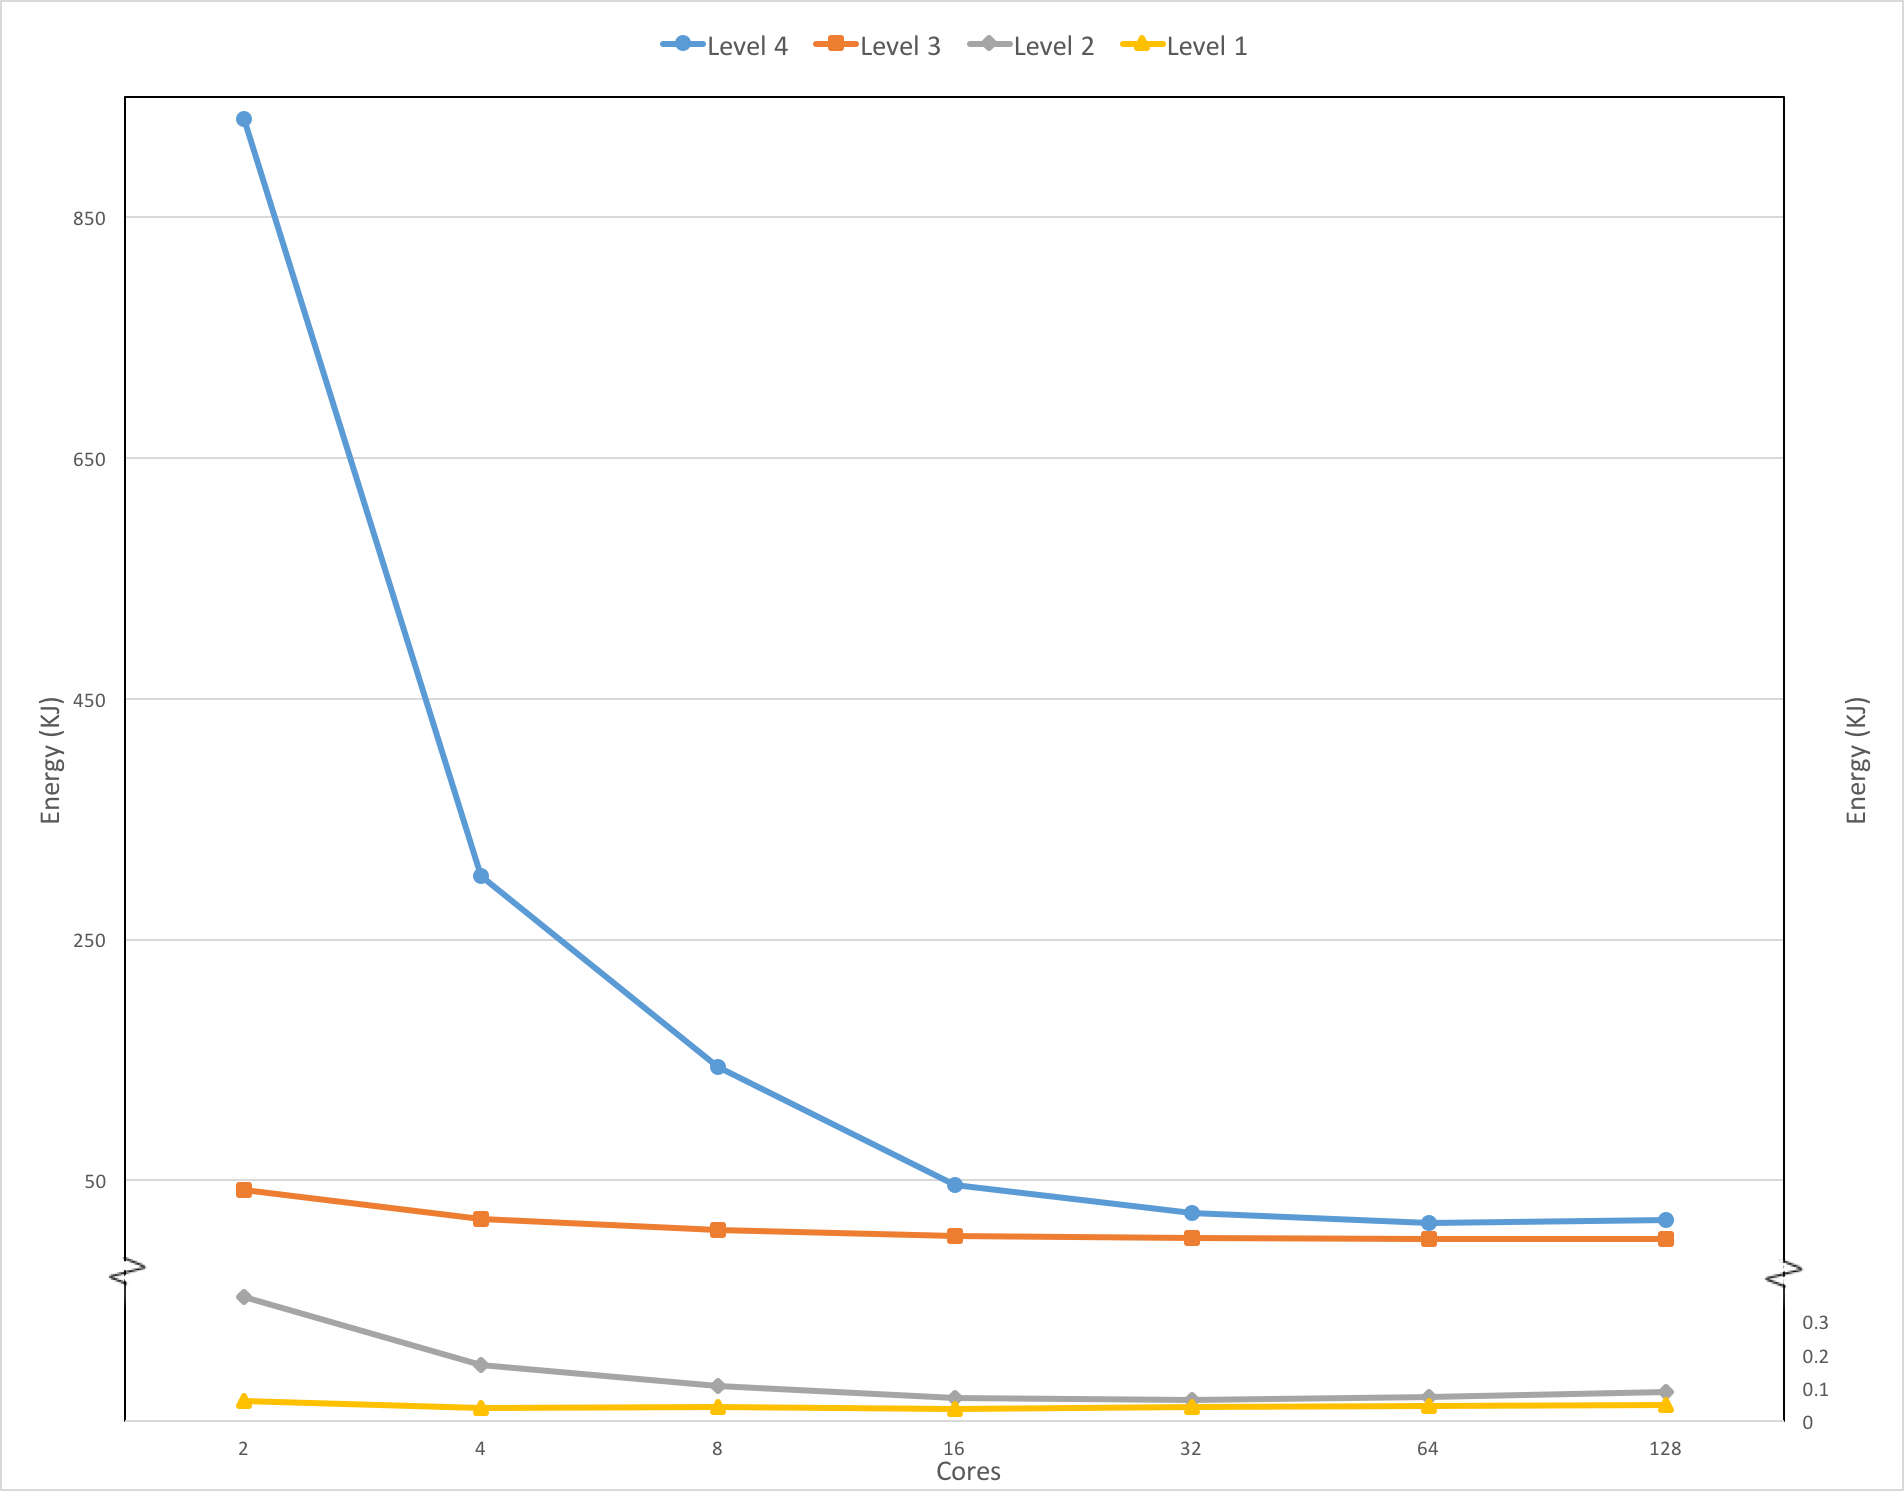
\includegraphics[width=8cm]{figs/CAPER_lev1-4_power_edited.jpg}
        \caption{Power consumption of different levels of refinement under different number of cores }
        \label{fig:powerconsumptioncaper}
\end{figure}

\noindent
%\textbf{Discussion}

Figure \ref{fig:powerconsumptioncaper} shows that there is a huge energy difference on the beginning of this curve. When running on 2 cores, the highest one (level 4) consumes almost 930 KJ while the lowest one (level 1) only take around 0.6 KJ. Since this experiment measure the all 8 node processors power status, the huge energy consumption of level 4 comes from the long execution time. It takes 1,314 seconds to run level 4 job while only 10 seconds to execute level 1. Most energy consumption comes from processors in idle state. But when assign appropriate processor resources to it, the curve reaches the flat zoom, the energy consumption difference is reasonable and stable. From this point of view, an appropriate number of cores for a certain workload is very crucial for energy consumption.



\subsubsection{Evaluation of the impact of RAPL power capping on LMC performance }
This experiment is aimed at studying the impact of power capping on LMC power-performance. And it would also give us a reference about the optimal power capping setting for different resolution levels. 


%\noindent
%\textbf{Methodology}

We use level 1 to level 4 in LMC as inputs to measure the time and power consumption. Since CAPER CPU power is 95W (Intel Xeon E5-2650 V2), in this experiment, we cap the CPU power to 25W, 35W, 45W, 55W, 65W, 75W, 85W, and 95W and record the package energy consumption (PKG) and execution time respectively. Package energy consumption is the energy used by the CPU chip itself including cores, caches and graphics, etc. 


\noindent
\textbf{Configuration}
\begin{table}[H]
\begin{center}
\begin{tabular}{|l|l|}
	\hline
	\textbf{Parameter} & \textbf{Value}\\ \hline
    Platform & CAPER cluster\\ 		\hline
    Number of cores & 64 cores\\
	\hline
    Level of refinement  & level 1 to level 4\\
    \hline
    Time step & 10\\
    \hline
    Time unit & Second\\
    \hline
    Power measurement object & 8 nodes processors\\
    \hline
    Power capping & 95W to 25W decrease by 10\\
    \hline
    RAPL sample rate & 2 Hz\\
    \hline
\end{tabular}
\end{center}
\caption{Configuration for experiment of exploring the affection of RAPL power capping on LMC performance 
}
\label{table:table_rapl_capping}
\end{table}

%\textbf{Power capping with RAPL}\\
We use Intel \textit{power\_gadget} tool to cap the power. To use it, we assign value to the parameter \textit{MY\_POWER\_LIMIT}, then compile and run it.
We use linux command line ``time'' to measure the execution time. The execution command line is provided as follows:
%\begin{adjustwidth}{2cm}{4cm}
time mpirun -machinefile hostfile.txt -np 64 .\/LMC2d.Linux.g++.gfortran.SDC.MPI.ex inputfile amr.max\_lev=\#level
%\end{adjustwidth}

For the power measurement, we also use the Intel \textit{power\_gadget} tool. When running it, it will give the real-time power consumption data every 0.5 second.



\noindent
%\textbf{Result}
\begin{figure}[H]
	\centering
    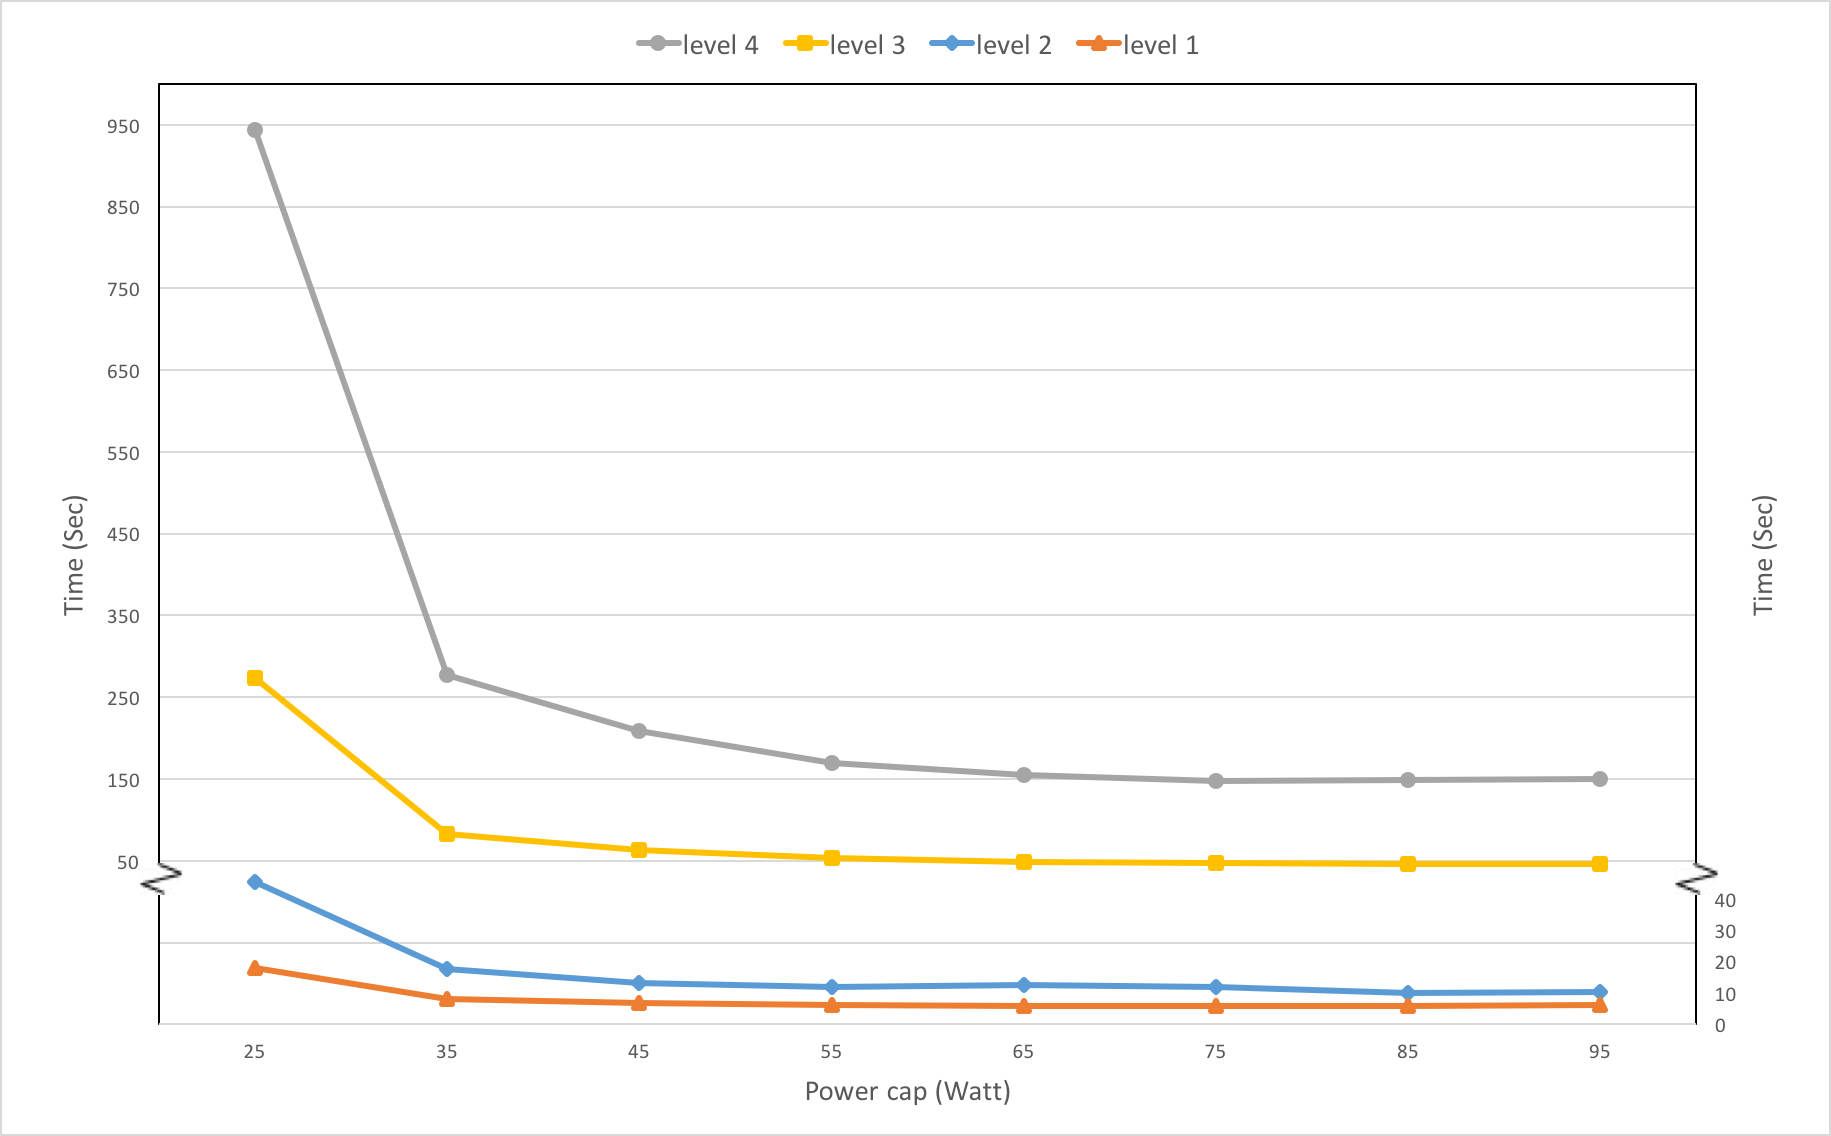
\includegraphics[width=8cm]{figs/CAPER_lev1-4_power_cap_time_edited.png}
        \caption{Relationship between different resolution of LMC and their execution time under different power capping levels}
        \label{fig:RAPLpowercaptime}
\end{figure}

\begin{figure}[H]
	\centering
    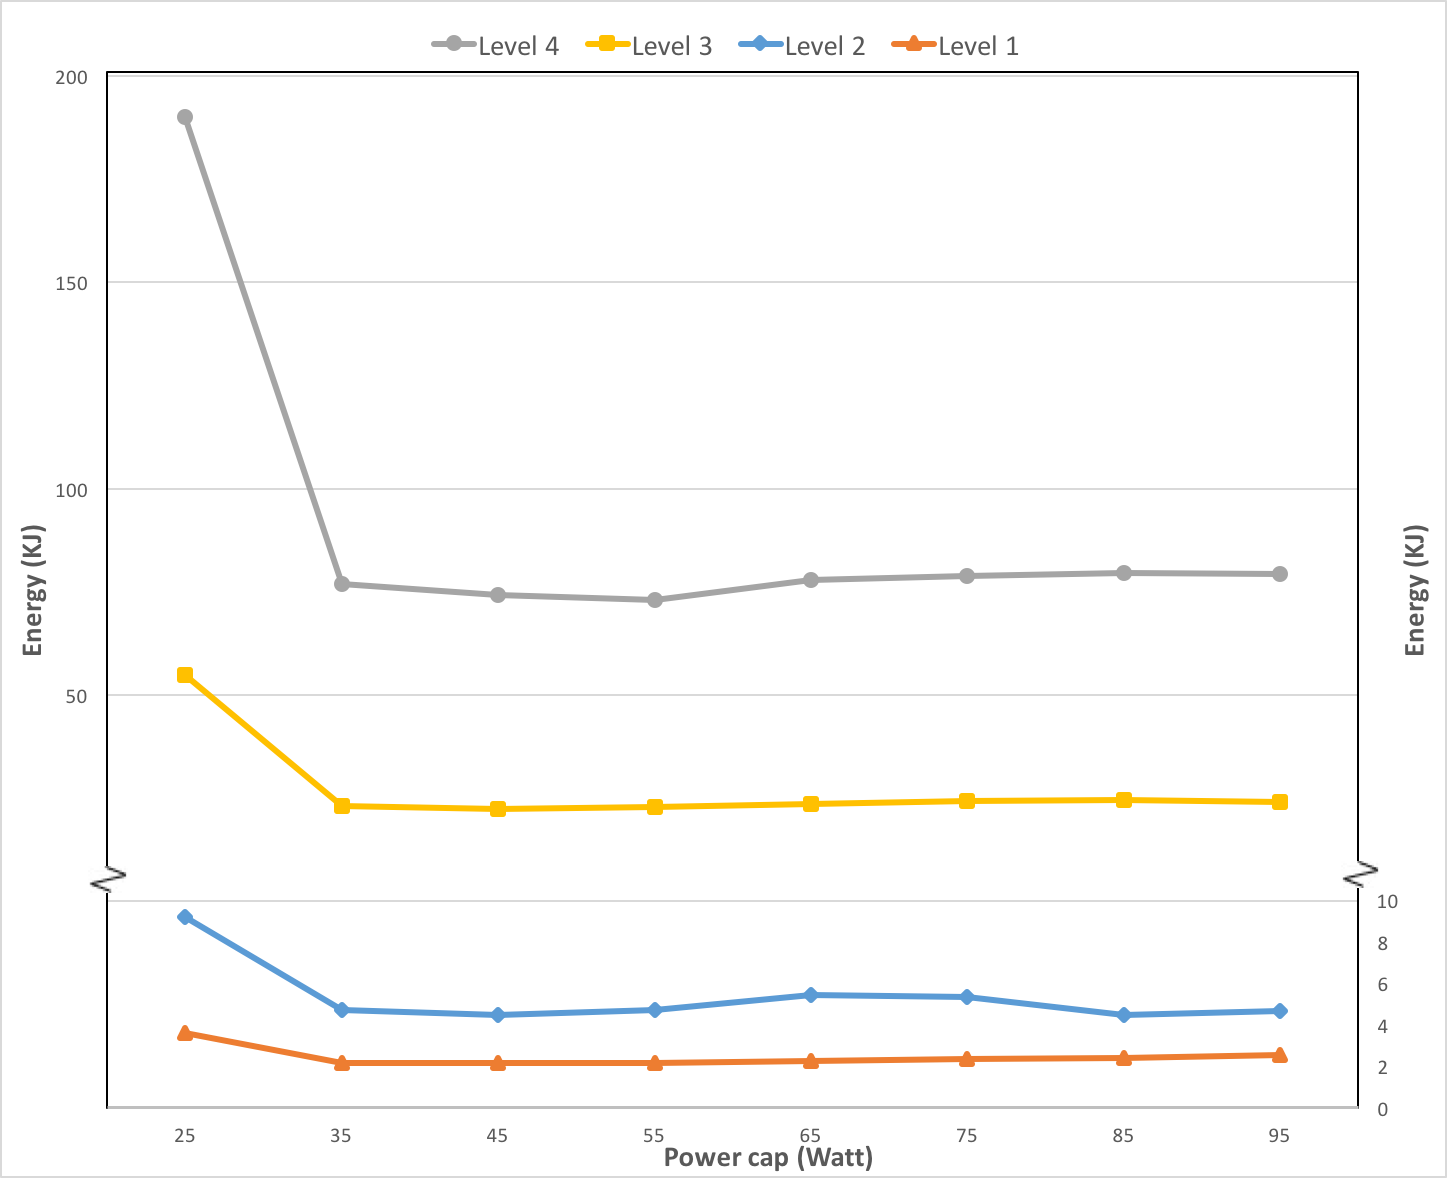
\includegraphics[width=8cm]{figs/CAPER_lev1-4_power_cap_energy_edited.png}
        \caption{Relationship between different resolution of LMC and the energy consumption under different power capping levels}
        \label{fig:RAPLpowercappower}
\end{figure}

\noindent
%\textbf{Discussion}

Figure presents the energy consumption result of executing level 1 to level 4 LMC program on certain number of cores under different power capping configurations. Those curves have the same pattern that sharply decreasing from 25 to 35 and becoming flat between 65 and 95. The lowest energy consumption is appearing when CPU power was capped to 45W to 55W. This can be explaining from execution data that without any CPU power capping, LMC program will boots CPU to 65W to 75W during execution whatever executing on how many cores. This also can be seem from the flat curve on segment 65W to 95W on each chart. Therefore, the advantage of power capping is working when CPU power down below 65W, and optimize between 45W to 55W. 



\subsubsection{Evaluation of power budget acquisition through power capping and resolution degradation}
The previous experiments have characterized the behavior of LMC. It can be concluded that the execution time will increase as the level of refinement/resolution increases or CPU power is capped down. Also, the energy consumption trend for different power caps and refinement levels is shown in Figure \ref{fig:Energy_consumption_trend}. The energy consumption presents the same trend as the execution time, i.e., LMC will consume more energy as the levels of refinement/resolution increase or capping down CPU power. The question here is how to use this characterization to create available power budget. We propose to combine these two factors, adjusting resolution and applying appropriate power capping, to get available power budget for running other tasks (e.g., checkpointing). 


\textbf{Configuration}
\begin{table}[H]
\begin{center}
\begin{tabular}{|l|l|}
	\hline
	\textbf{Parameter} & \textbf{Value}\\ \hline
    Platform & CAPER cluster\\ 		\hline
    Number of cores & 64 cores\\
	\hline
	Resolution & level 3 2 1\\
    \hline
    Time step & 10\\
    \hline
    Time unit & Second\\
    \hline
    Power measurement & RAPL meter\\
    \hline
    Power cap & RAPL\\
    \hline
\end{tabular}
\end{center}
\caption{Configuration for experiment of getting available power budget through power capping and resolution degradation
}
\label{table:table_tradeoff}
\end{table}



\begin{figure}[H]
	\centering
    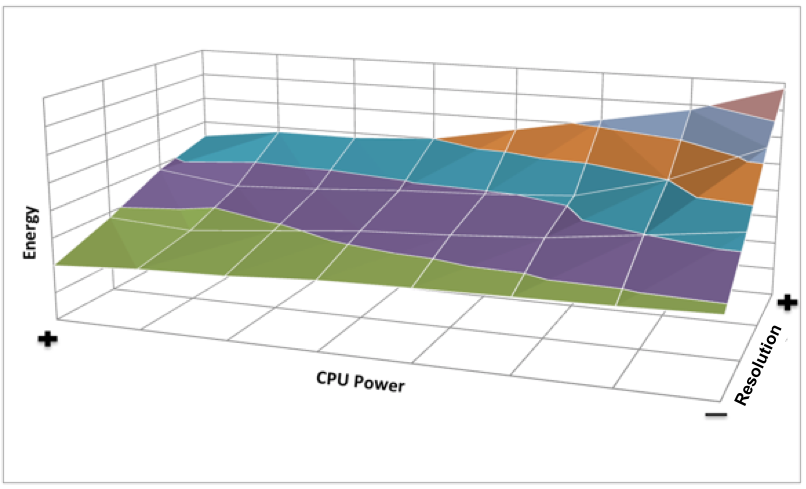
\includegraphics[width=8cm]{figs/Energy_consumption_trend.png}
        \caption{Energy consumption trend for different power caps and refinement levels}
        \label{fig:Energy_consumption_trend}
\end{figure}

\begin{figure}[H]
	\centering
    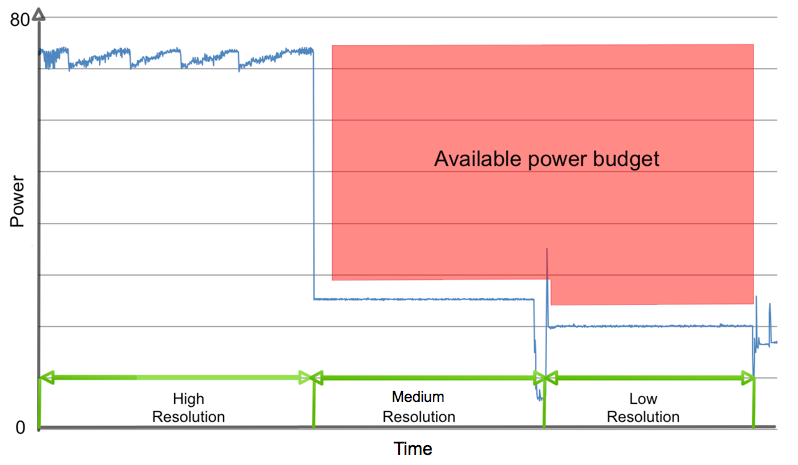
\includegraphics[width=8cm]{figs/Available_power_budget.png}
        \caption{Available power budget from applying resolution degradation and appropriate power capping}
        \label{fig:Available_power_budget}
\end{figure}


In previous Figure \ref{figs:LMCruntime}, we measured the power consumption of running LMC with different resolution. It shows that the execution time decreases when decreasing the resolution. Therefore, we apply appropriate power capping to the medium and low resolution execution to make their execution equal the execution time in highest resolution. As shown in Figure \ref{fig:Available_power_budget}, the red region is the available power budget extracted from the total power budget. 



\subsubsection{Evaluation of power budget management}
We have tested the impact of power capping and level of refinement of LMC on the performance and energy consumption. We also observed the potential power saving from degrading resolution and implementing power capping. The goal of this experiment is being able to use power budgets opportunistically for running other tasks. In the experiment, we propose to use this power budget to do  checkpointing, which will increase the resilience and make the LMC program running more reliably. 

In this experiment, we are proposing to degrade LMC resolution and cap its running power, then use this power budget to do check pointing. However, there are some limitations due to the code characteristics: (i) we can not separate the checkpoint function from simulation program, and (ii) we can not dynamically control LMC resolution. 

%\textbf{Methodology}\\
To address these two issues, we use two LMC executions running alternatively on two set of nodes to emulate one execution dynamically adjusting resolution and doing checkpoint. Each set of nodes contains three nodes for execution. When the first execution start doing checkpoint then the second set start another execution with lower resolution. We focus on system level power consumption. 

We implement this using a flag to coordinate these two LMC executions. We've recompiled the first LMC set program to let it write flag when it start to do checkpoint, and the second LMC set keeps reading the flag to start running when the flag turn to be true. As shown in Figure \ref{fig:lev3withoutpowercap}, when the blue curve is the first instance (set 1) of LMC finishes its execution, it triggers the second instance (set 2), which is the orange curve. Once the second instance is completed the first one is triggered again and so on. By doing this, we can emulate a single LMC execution running and dynamically change the resolution while giving the available power budget for doing checkpoint.



\textbf{Configuration}
\begin{table}[H]
\begin{center}
\begin{tabular}{|l|l|}
	\hline
	\textbf{Parameter} & \textbf{Value}\\ \hline
    Platform & CAPER cluster\\ 		\hline
    Number of cores & 64 cores\\
	\hline
    Resolution & level 4 3\\
    \hline
    Time step & 10\\
    \hline
    Time unit & Second\\
    \hline
    Power measurement object & 3 nodes processors\\
    \hline
    Power cap & RAPL\\
    \hline
\end{tabular}
\end{center}
\caption{Configuration for experiment of exploring the power-performance tradeoffs 
}
\label{table:table_tradeoff}
\end{table}



\begin{figure}[H]
	\centering
    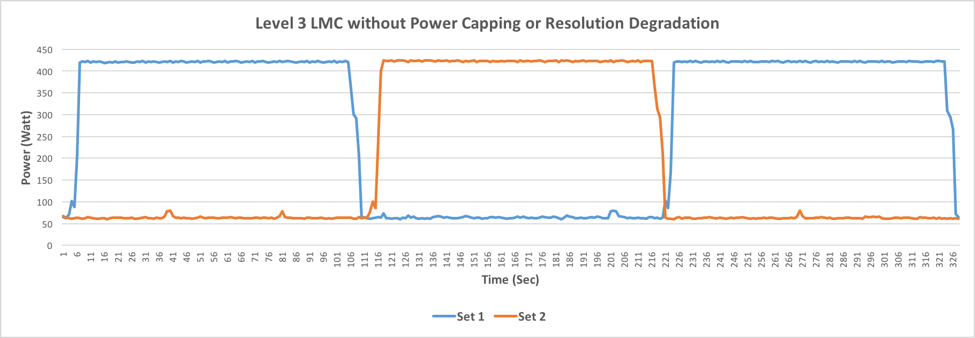
\includegraphics[width=8cm]{figs/lev3withoutpowercap.png}
        \caption{Level 3 LMC power consumption without power capping or resolution degradation}
        \label{fig:lev3withoutpowercap}
\end{figure}


\begin{figure}[H]
	\centering
    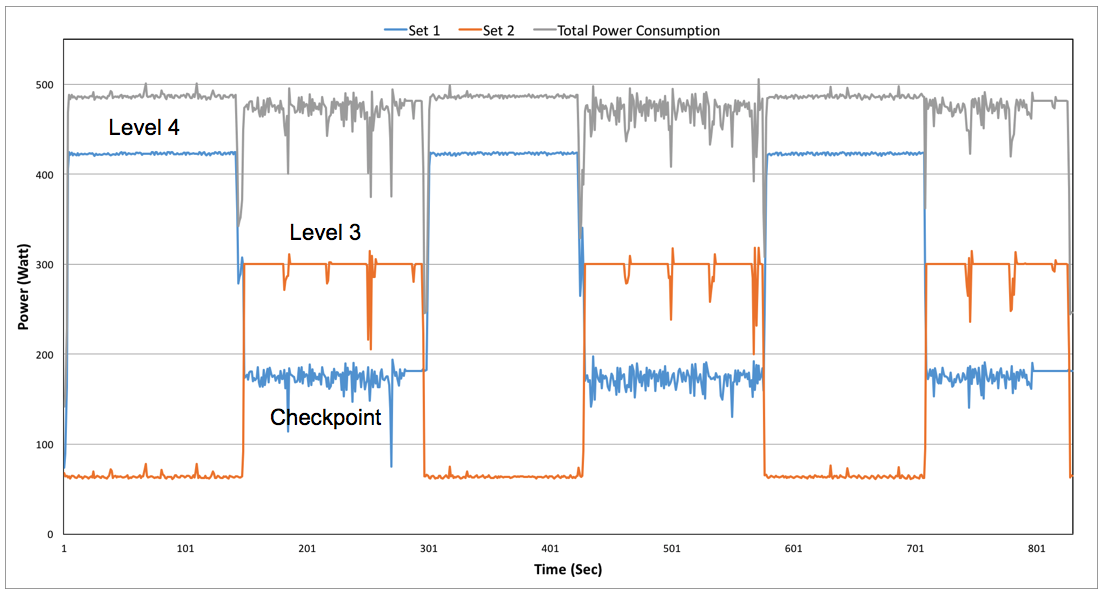
\includegraphics[width=8cm]{figs/LMCtradeoff.png}
        \caption{Level 4 LMC power consumption with power capping or resolution degradation}
        \label{fig:LMCtradeoff}
\end{figure}

In Figure \ref{fig:LMCtradeoff}, the blue curve is the set 1 running the high resolution LMC (level 4). Once it starts doing checkpointing, the set 2 (in orange curve) is triggered to run LMC at level 3. Configuring power capping appropriately, the total power consumption, which is shown in gray curve on the top, is kept constant. This means we successfully constraint the power budget of LMC to perform other tasks (i.e., checkpointing).
